\documentclass{article}

\usepackage{tikz}
\usepackage{booktabs}
\usepackage[margin={2cm,1.5cm}]{geometry}

\title{IsaFoR Sessions and Heap Images}
\date{April 29, 2025}

\begin{document}
\maketitle

\section*{Session and Heap Image Graph}

The dependencies have been manually extracted from the ROOT file,
ignoring the dependencies of HOL-Lib and HOL-AFP.

The dependencies in the diagram are logical and do not include
dependencies that are enforced via the build-process.

The heap-image sessions IsaFoR\_\{1,2,3\} are indicated by the rectangles.

\begin{center}
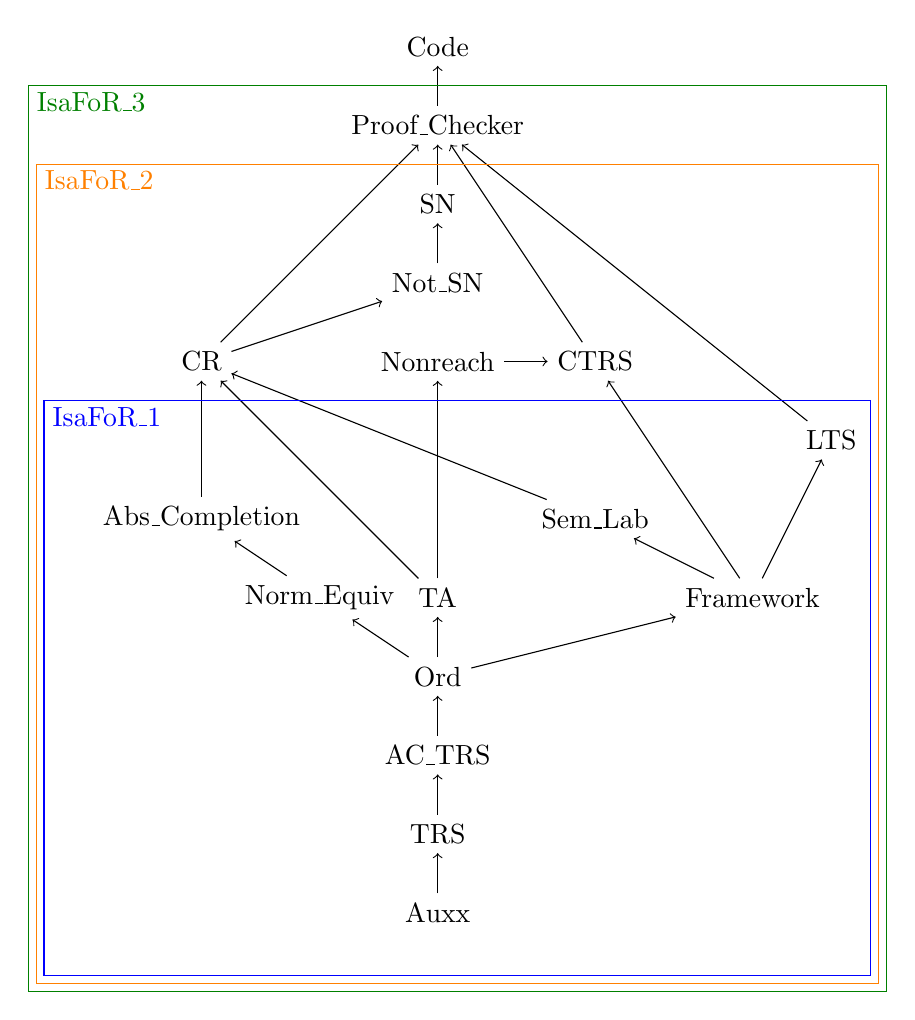
\begin{tikzpicture}
\node (aux) at (4,-1) {Auxx};
\node (trs) at (4,0) {TRS};
\node (ac) at (4,1) {AC\_TRS};
\node (ord) at (4,2) {Ord};
\node (ta) at (4,3) {TA};
\node (frame) at (8,3) {Framework};
\node (ne) at (2.5,3) {Norm\_Equiv};
\node (semlab) at (6,4) {Sem\_Lab};
\node (nr) at (4,6) {Nonreach};
\node (abscomp) at (1,4) {Abs\_Completion};
\node (lts) at (9,5) {LTS};
\node (ctrs) at (6,6) {CTRS};
\node (cr) at (1,6) {CR};
%\node (lisa) at (2.5,7) {Lisa};
\node (nsn) at (4,7) {Not\_SN};
\node (sn) at (4,8) {SN};
\node (pc) at (4,9) {Proof\_Checker};
\node (code) at (4,10) {Code};

\draw [->] (aux) -- (trs);
\draw [->] (trs) -- (ac);
\draw [->] (ord) -- (ta);
\draw [->] (ac) -- (ord);
\draw [->] (ord) -- (ne);
\draw [->] (ord) -- (frame);
\draw [->] (ta) -- (nr);
\draw [->] (nr) -- (ctrs);
\draw [->] (frame) -- (ctrs);
\draw [->] (frame) -- (lts);
\draw [->] (frame) -- (semlab);
\draw [->] (ne) -- (abscomp);
\draw [->] (semlab) -- (cr);
\draw [->] (ta) -- (cr);
\draw [->] (abscomp) -- (cr);
%\draw [->] (cr) -- (lisa);
%\draw [->] (lisa) -- (pc);
\draw [->] (cr) -- (pc);
\draw [->] (cr) -- (nsn);
\draw [->] (nsn) -- (sn);
\draw [->] (sn) -- (pc);
\draw [->] (lts) -- (pc);
\draw [->] (ctrs) -- (pc);
\draw [->] (pc) -- (code);

\draw[blue] (-1,-1.8) rectangle (9.5,5.5) node at (-0.2,5.3) {\mbox{IsaFoR\_1}};
\draw[orange] (-1.1,-1.9) rectangle (9.6,8.5) node at (-0.3,8.3) {\mbox{IsaFoR\_2}};
\draw[green!50!black] (-1.2,-2) rectangle (9.7,9.5) node at (-0.4,9.3) {\mbox{IsaFoR\_3}};
\end{tikzpicture}
\end{center}

\section*{Heap Image Information}
The following table presents information on the number of theories in the heap image
as well as the expected build time in format mm:ss.
The theories have been compiled %(using -v) 
with Isabelle 2025 and corresponding AFP.

\begin{center}
\begin{tabular}{lrrrrrrr}
\toprule
               & HOL-Lib  & HOL-AFP & IsaFoR\_1 & IsaFoR\_2 & IsaFoR\_3 & Code\\
%\# theories    & 147      & 463     & 199       & 170       & 26        & 1 \\                         
\midrule
Apple M1 Pro, 32 GB: 
               & 4:48     & 10:14    & 7:38      & 6:58      & 7:53      & 4:39 \\
Apple M2 Max, 64 GB:
               & 4:03     &  8:00    & 5:12      & 5:20      & 6:50      & 4:08 \\               
%8-Core Intel Xeon W, 64 GB:
%               & :     & :   & :      & :     & :     & :  \\               
\bottomrule
\end{tabular}
\end{center}

\end{document}
